\chapter{病毒学}\label{ch:b3:virology}

地球上大约有 $10^{31}$ 个\omterm{def:b3:virology:virus}{病毒}颗粒，平均每个细胞对应十个，
而在海洋中，它们每天杀死全部细菌的五分之一。\omterm{def:b3:virology:virus}{病毒}
不是细胞：它没有代谢，没有核糖体，无法
自行制造任何东西。它是一段基因组——短者仅两个基因，长者可达
两千个基因——外包蛋白质外壳，进入细胞后，把细胞的机器
转而用于复制它自身。1918 年的流感
夺去五千万人的生命；天花仅在二十世纪便夺去三亿
人的生命，并于 1980 年被一种
1796 年首次试用的\omterm{def:b3:virology:drugs}{疫苗}根除；而一种传入人类的冠状\omterm{def:b3:virology:virus}{病毒}
于 2019 年出现，数周内完成基因组测序，数日内设计出\omterm{def:b3:virology:drugs}{疫苗}，
并于两年内研制出针对其蛋白酶的药物。本
章讨论\omterm{def:b3:virology:virus}{病毒}是什么，以及如何依据其基因组的
化学性质对其分类，它们如何增殖，单一宿主内感染的动力学——
一对微分方程足以很好地描述它，并已改变了
艾滋病的治疗——它们的演化，
以及如何与之对抗。

\section{病毒是什么}

\begin{definition}[病毒]\label{def:b3:virology:virus}
\index{病毒}\index{衣壳}\index{包膜}\index{病毒粒子}\index{巴尔的摩分类}
\emph{病毒}是一种专性细胞内寄生物，由
核酸基因组构成——DNA 或 RNA，单链或双链，线状
或环状，单分子或多分子——包装于蛋白质
\emph{衣壳}之中，多数情况下还包有取自宿主膜的\emph{包膜}，
包膜上嵌有病毒糖蛋白。完整的
感染性颗粒即为\emph{病毒粒子}，多数直径为 \qtyrange{20}{300}{nm}
（少数巨型病毒可达一微米）。衣壳
由许多拷贝的一种或几种蛋白质，按
螺旋对称（棒状，如烟草花叶病毒）或二十面体对称（
即 $60T$ 个亚基构成的外壳，$T = 1, 3, 4, 7,\dots$）排列。\emph{巴尔的摩
分类}对病毒分组，依据由基因组到信使 RNA
的途径分为：I，双链 DNA（疱疹病毒、痘病毒、腺病毒、多数噬菌体）；II，
单链 DNA（细小病毒）；III，双链 RNA（轮状病毒）；
IV，正链 RNA，本身即是信使 RNA（脊髓灰质炎病毒、丙型肝炎病毒、
冠状病毒）；V，负链 RNA，与信使 RNA 互补
（流感病毒、麻疹病毒、狂犬病病毒、埃博拉病毒）；VI，RNA 逆转录为
DNA（逆转录病毒，即 HIV）；VII，DNA 经 RNA 中间体复制
（乙型肝炎病毒）。除 I 类外，每一类都必须携带或编码一种细胞所缺乏的
酶，如 RNA 依赖的 RNA 聚合酶和逆转
录酶——这些酶正是多数\omterm{def:b3:virology:drugs}{抗病毒
药物}的靶点。
\end{definition}

\begin{proof}[证据]
伊万诺夫斯基（1892）和拜耶林克（1898）证明烟草的花叶病
可由通过滤器的汁液传染，该滤器截留了全部
细菌——一种\emph{contagium vivum fluidum}，即活的传染性液体。
斯坦利（1935）将病原体，即烟草花叶\omterm{def:b3:virology:virus}{病毒}，结晶出来，
并证明它是蛋白质，其中（如鲍登和皮里所发现）含 \qty{5}{\%}
RNA。赫尔希和蔡斯（1952）用 $^{35}$S 标记噬菌体的蛋白质
，用 $^{32}$P 标记其 DNA，使之侵染\emph{E.~coli}，
用搅拌器剪去空的外壳，发现 $^{32}$P 在
细胞内，$^{35}$S 在细胞外：DNA 进入细胞，而蛋白质
留在外面，因此 DNA 携带遗传指令。弗兰克尔-科内特
（1955）将烟草花叶\omterm{def:b3:virology:virus}{病毒}拆分为蛋白质和 RNA，
再用一株系的 RNA 和另一株系的蛋白质重组出感染性颗粒；
其子代属于 RNA 所属的株系。
\end{proof}

\begin{proposition}[遗传经济性：为何衣壳是对称的]\label{prop:b3:virology:economy}
\index{遗传经济性}
\omterm{def:b3:virology:virus}{衣壳}必须包裹编码它的基因组。质量为 $m$ 的蛋白质
约需 $m/\qty{110}{Da}$ 个密码子，即 $3m/110$ 个核苷酸，
一段 RNA 约重 $3m/110\times\qty{330}{Da} = 9m$：任何
蛋白质都由其自身九倍质量的核酸编码。一个外壳
由\emph{单个}蛋白质分子构成、包裹基因组，
就须包裹其自身九倍质量的基因组，仅为编码自身，并且
外壳无法在生物学密度下容纳其自身九倍质量的核酸。
解决之道由克里克和沃森（1956）指出，即
用许多拷贝的同一种小蛋白质构成外壳：烟草花叶\omterm{def:b3:virology:virus}{病毒}
以其基因组中 \qty{480}{nt} 的区段编码一种 \qty{17.5}{kDa} 的外壳蛋白，
该基因组全长 \qty{6400}{nt}，外壳由 $2130$ 个拷贝组成。
完全相同的亚基以相同方式堆积，必然按对称方式排列，因此\omterm{def:b3:virology:virus}{病毒}\omterm{def:b3:virology:virus}{衣壳}
或为螺旋体，或为二十面体，同样的经济性也使其
具备自\omterm{def:b3:genomics:assembly}{组装}的能力，因为每个亚基只需识别其
相邻亚基。
\end{proposition}
\begin{proof}
质量比由一个密码子含三个核苷酸，每个约
\qty{330}{Da}，而一个残基约 \qty{110}{Da} 推得：$3\times 330/110 =
9$。由单个 \qty{40}{MDa} 蛋白质构成的\omterm{def:b3:virology:virus}{衣壳}将包裹 \qty{360}{MDa}
的核酸，相当于核酸密度下半径约 \qty{50}{nm} 的球体，
而蛋白质本身构成的外壳厚度约为
\qty{2}{nm}，半径相同——几何上可行，
但一条由 $360\,000$ 个残基组成、能正确折叠的单一多肽
并不可能，且一个突变即可使其失效。若有 $n$ 个相同亚基，
编码成本减少为原来的 $n$ 分之一，而包围的体积不变。
\end{proof}

\begin{omfigure}
\begin{tikzpicture}[every node/.style={font=\scriptsize}, >=stealth]
  \node[draw, thick, rounded corners, fill=omMeth!30, minimum width=2.4cm] (mrna) at (0,0) {mRNA $\to$ 蛋白质};
  \node[draw, thick, rounded corners, fill=omDef!20, align=center] (I) at (-5.8,3.6) {I：dsDNA\\疱疹病毒、痘病毒、T4 噬菌体};
  \node[draw, thick, rounded corners, fill=omDef!20, align=center] (II) at (-2.0,3.6) {II：ssDNA\\细小病毒};
  \node[draw, thick, rounded corners, fill=omThm!20, align=center] (III) at (2.0,3.6) {III：dsRNA\\轮状病毒};
  \node[draw, thick, rounded corners, fill=omThm!20, align=center] (IV) at (5.8,3.6) {IV：(+)RNA\\脊髓灰质炎病毒、丙型肝炎病毒、\\冠状病毒};
  \node[draw, thick, rounded corners, fill=omThm!20, align=center] (V) at (-5.6,-3.4) {V：($-$)RNA\\流感病毒、麻疹病毒、\\狂犬病病毒、埃博拉病毒};
  \node[draw, thick, rounded corners, fill=omProp!30, align=center] (VI) at (0,-3.4) {VI：RNA $\to$ DNA\\逆转录病毒（HIV）};
  \node[draw, thick, rounded corners, fill=omProp!30, align=center] (VII) at (5.6,-3.4) {VII：DNA 经 RNA 途径 \\乙型肝炎病毒};
  \node[below, font=\tiny, align=center, gray!50!black] at (-5.8,2.9) {宿主 RNA 聚合酶};
  \node[below, font=\tiny, align=center, gray!50!black] at (-2.0,3.05) {合成第二条链，\\随后转录};
  \node[below, font=\tiny, align=center, gray!50!black] at (2.0,3.05) {病毒 RNA 聚合酶 \\位于颗粒内};
  \node[below, font=\tiny, align=center, gray!50!black] at (5.8,2.75) {基因组即为 mRNA};
  \node[above, font=\tiny, align=center, gray!50!black] at (-5.6,-2.55) {病毒聚合酶复制它};
  \node[above, font=\tiny, align=center, gray!50!black] at (0,-2.85) {逆转录酶、整合，\\随后宿主聚合酶};
  \node[above, font=\tiny, align=center, gray!50!black] at (5.6,-2.85) {DNA 的转录};
  \foreach \c in {I,II,III,IV,V,VI,VII} \draw[->, thick] (\c) -- (mrna);
\end{tikzpicture}

{\small \omterm{def:b3:virology:virus}{巴尔的摩分类}的七类，按从基因组到
信使 RNA 的途径排列。除 I 类外，每一类都需要宿主细胞不提供的
一种酶——这正是\omterm{def:b3:virology:drugs}{抗病毒药物}的天然靶点。}
\end{omfigure}

\begin{omfigure}
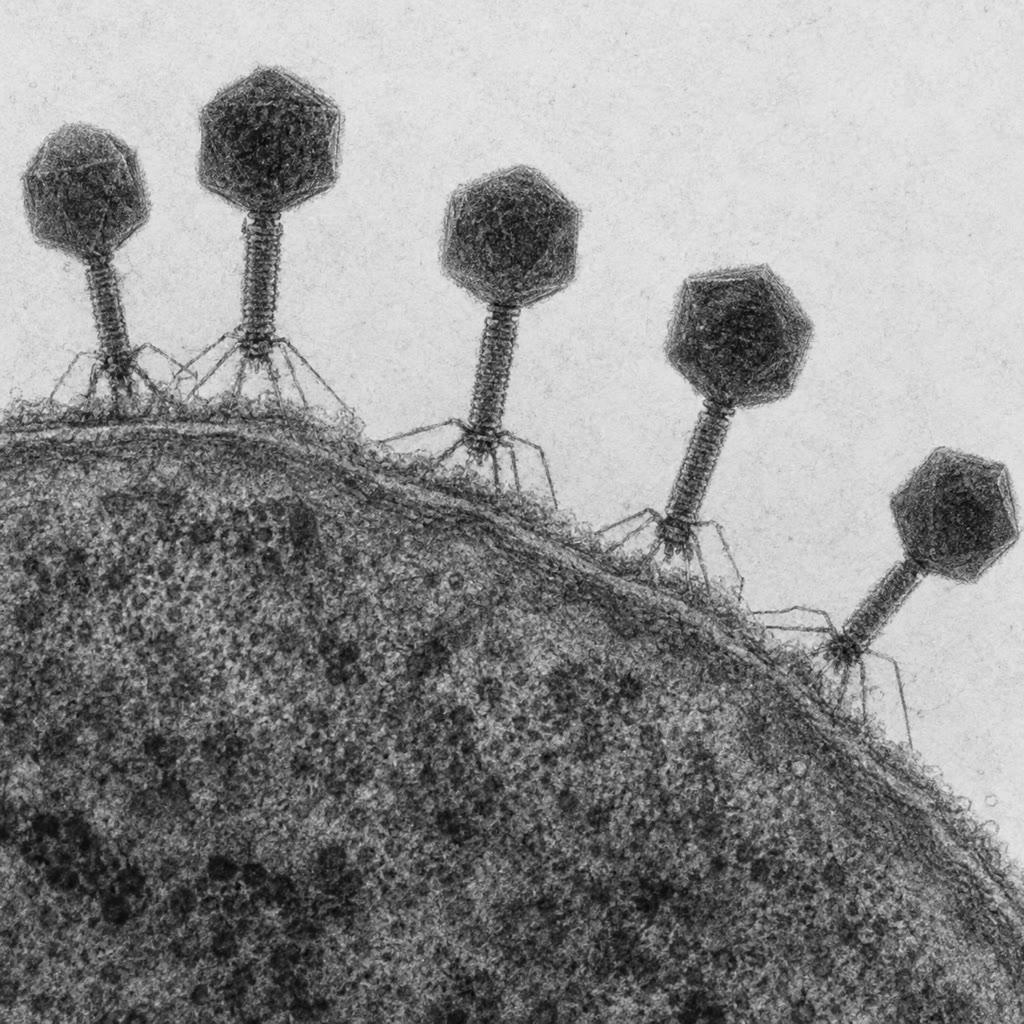
\includegraphics[width=0.36\linewidth]{images/book5/ai/b5-13-phage-tem.jpg}\hspace{0.04\linewidth}
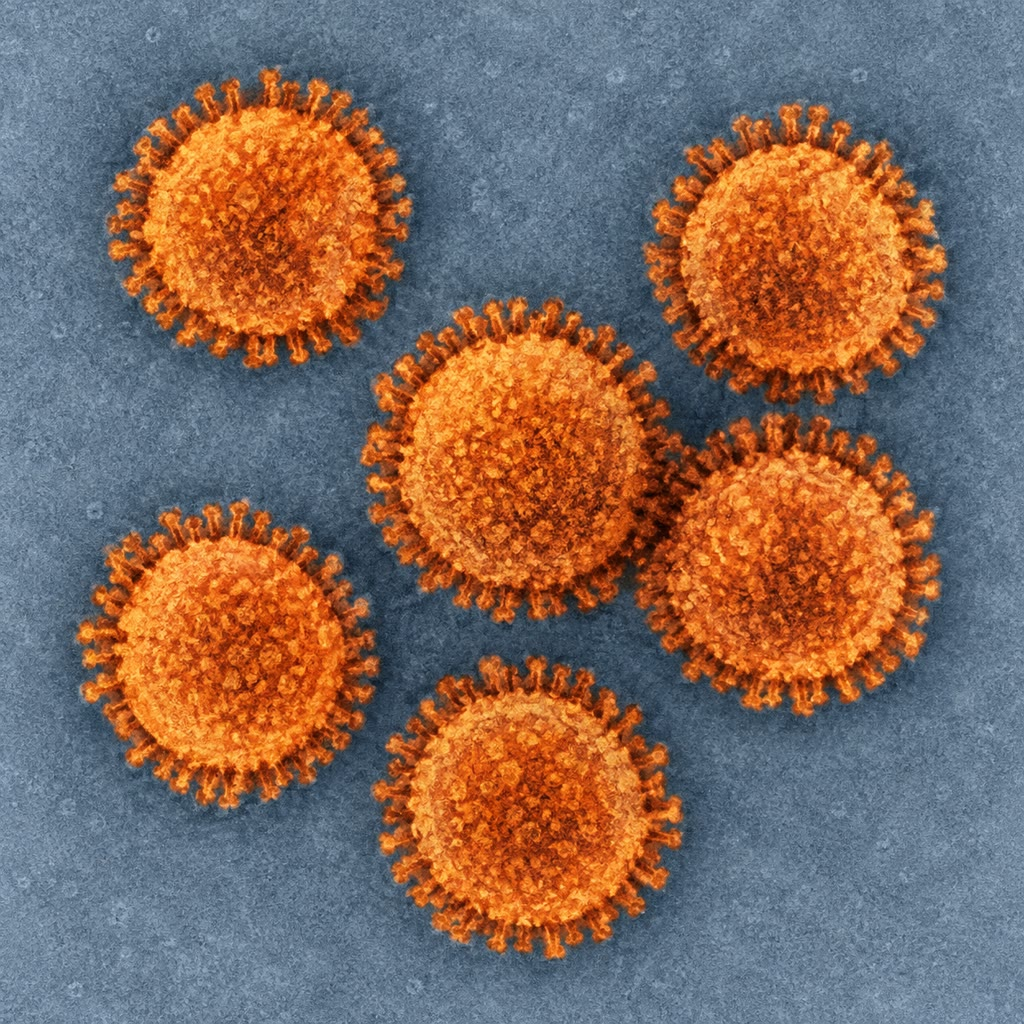
\includegraphics[width=0.36\linewidth]{images/book5/ai/b5-13-influenza-virions.jpg}

{\small 左：噬菌体借尾丝附着于
细菌，每个头部为由 DNA 构成的二十面体\omterm{def:b3:virology:virus}{衣壳}。右：流感\omterm{def:b3:virology:virus}{病毒
粒子}，有\omterm{def:b3:virology:virus}{包膜}，其表面布满血凝素与
神经氨酸酶刺突。}
\end{omfigure}

\section{病毒如何增殖}

\begin{definition}[复制周期]\label{def:b3:virology:cycle}
\index{病毒复制周期}\index{受体!病毒}\index{溶原性}\index{潜伏}
每种\omterm{def:b3:virology:virus}{病毒}都经历相同的阶段。\emph{吸附}：与特定宿主受体结合——
HIV 为 CD4 和一种趋化因子受体，
SARS 冠状\omterm{def:b3:virology:virus}{病毒}为 ACE2，流感\omterm{def:b3:virology:virus}{病毒}为唾液酸，噬菌体为
\omterm{def:b3:bacteriology:envelope}{脂多糖}或孔蛋白——这决定了\omterm{def:b3:virology:virus}{病毒}能感染哪些
物种与哪些细胞（其\emph{嗜性}）。
\emph{进入}：\omterm{def:b3:virology:virus}{包膜}与质\omterm{def:b3:membrane-traffic:fusion}{膜融合}，或
经胞吞作用后在酸性\omterm{def:b3:membrane-traffic:endocytosis}{内体}内融合，或对
噬菌体而言，基因组穿过细胞壁注入。\emph{脱壳}，
\omterm{def:b3:virology:virus}{病毒}基因按各类的特定途径\emph{表达}，以及
基因组的\emph{复制}，常在\omterm{def:b3:virology:virus}{病毒}构建的“工厂”内进行，
位于细胞质或细胞核中。新\omterm{def:b3:virology:virus}{衣壳}围绕新基因组的\emph{\omterm{def:b3:genomics:assembly}{组装}}，
由对称亚基的自\omterm{def:b3:genomics:assembly}{组装}驱动，以及
\emph{释放}：通过细胞裂解，或通过出芽穿过膜，
后者同时提供\omterm{def:b3:virology:virus}{包膜}。有些\omterm{def:b3:virology:virus}{病毒}则可将自身
基因组插入宿主基因组并等待：噬菌体 $\lambda$ 的\emph{溶原性}，
其阻遏蛋白使之保持沉默，直至宿主受损；
疱疹\omterm{def:b3:virology:virus}{病毒}在神经元中的\emph{潜伏}可持续终身，HIV 则
以前\omterm{def:b3:virology:virus}{病毒}形式潜伏于静息 T~细胞中，
任何作用于复制的药物都无法将其清除。
\end{definition}

\begin{omfigure}
\begin{tikzpicture}[every node/.style={font=\scriptsize}, >=stealth]
  % cell
  \draw[very thick, omDef, fill=omDef!6] (0,0) ellipse (5.6 and 3.2);
  \draw[thick, omDef!70, fill=omDef!20] (1.8,0) ellipse (1.6 and 1.1); \node at (1.8,0.75) {细胞核};
  % virion outside
  \draw[thick, omProp, fill=omProp!30] (-7.2,1.6) circle (0.35); \foreach \a in {0,45,...,315} \draw[omProp, thick] (-7.2,1.6) ++(\a:0.35) -- ++(\a:0.15);
  \node[above] at (-7.2,2.1) {病毒粒子};
  \draw[->, thick] (-6.8,1.4) -- (-5.7,0.9); \node[below, align=center] at (-6.6,1.0) {1. 吸附于 \\受体};
  % entry
  \draw[thick, omProp] (-5.4,0.7) arc[start angle=140, end angle=40, radius=0.5];
  \node[below, align=center] at (-3.9,-0.2) {2. 融合或胞吞；\\3. 脱壳};
  % genome path
  \draw[omThm, very thick] (-3.4,0.2) .. controls (-2.6,0.6) .. (-1.8,0.4);
  \draw[->, thick] (-1.6,0.4) -- (-0.4,0.4);
  \node[above, align=center] at (-1.0,0.55) {4. 表达基因，\\复制基因组};
  \draw[omThm, very thick] (-1.0,-0.5) -- (0.4,-0.5); \draw[omThm, very thick] (-1.0,-0.75) -- (0.4,-0.75); \draw[omThm, very thick] (-1.0,-1.0) -- (0.4,-1.0);
  % assembly
  \foreach \p in {(1.2,-1.6),(1.9,-1.9),(2.6,-1.5)} { \draw[thick, omProp, fill=omProp!30] \p circle (0.25); }
  \node[below, align=center] at (1.9,-2.2) {5. 围绕基因组 \\组装衣壳};
  % budding
  \draw[thick, omProp, fill=omProp!30] (4.9,-1.7) circle (0.32); \draw[->, thick] (5.3,-1.75) -- (6.4,-2.0);
  \draw[thick, omProp, fill=omProp!30] (7.0,-2.2) circle (0.35); \foreach \a in {0,45,...,315} \draw[omProp, thick] (7.0,-2.2) ++(\a:0.35) -- ++(\a:0.15);
  \node[below, align=center] at (6.4,-2.6) {6. 穿膜出芽 \\（获得包膜）或裂解细胞};
  % latency
  \draw[->, thick, dashed, omMeth!70!black] (-0.2,0.2) -- (0.9,0.2); \node[below, omMeth!70!black, align=center, font=\tiny] at (2.0,-0.05) {逆转录病毒：整合 \\为前病毒；潜伏};
\end{tikzpicture}

{\small 有\omterm{def:b3:virology:virus}{包膜}\omterm{def:b3:virology:virus}{病毒}的复制周期：吸附于
受体，进入并脱壳，在宿主的
机制中表达与复制，\omterm{def:b3:genomics:assembly}{组装}，再经出芽释放——或对逆转录\omterm{def:b3:virology:virus}{病毒}而言，
整合进宿主基因组并保持沉默。}
\end{omfigure}

\begin{method}[计数感染性颗粒：噬斑试验]\label{met:b3:virology:plaque}
\index{噬斑试验}\index{滴度}
测定\omterm{def:b3:virology:virus}{病毒}储液：（1）以十倍梯度稀释；（2）将各稀释液
与过量宿主细胞混合——噬菌体用软琼脂中的细菌，
动物\omterm{def:b3:virology:virus}{病毒}用培养的单层细胞；（3）培养：
每个感染性颗粒感染一个细胞，子代再感染
邻近细胞，一两天后形成透明斑块，即\emph{噬斑}，
标记出\omterm{def:b3:virology:virus}{病毒}所在位置；（4）计数噬斑数在\numrange{30}{300}之间的平板，
乘以稀释倍数，即得以噬斑形成单位
（PFU）表示、每毫升的\emph{\omterm{met:b3:virology:plaque}{滴度}}。由于每个噬斑都是由一个颗粒克隆而来，
挑取噬斑即可获得纯的分离株。物理颗粒数
（经电子显微镜或 PCR 计数）与噬斑形成单位之比
通常远大于 1——对许多动物\omterm{def:b3:virology:virus}{病毒}而言为 10 至 1000 倍——
因为多数颗粒有缺陷或无法感染。
\end{method}

\begin{omfigure}
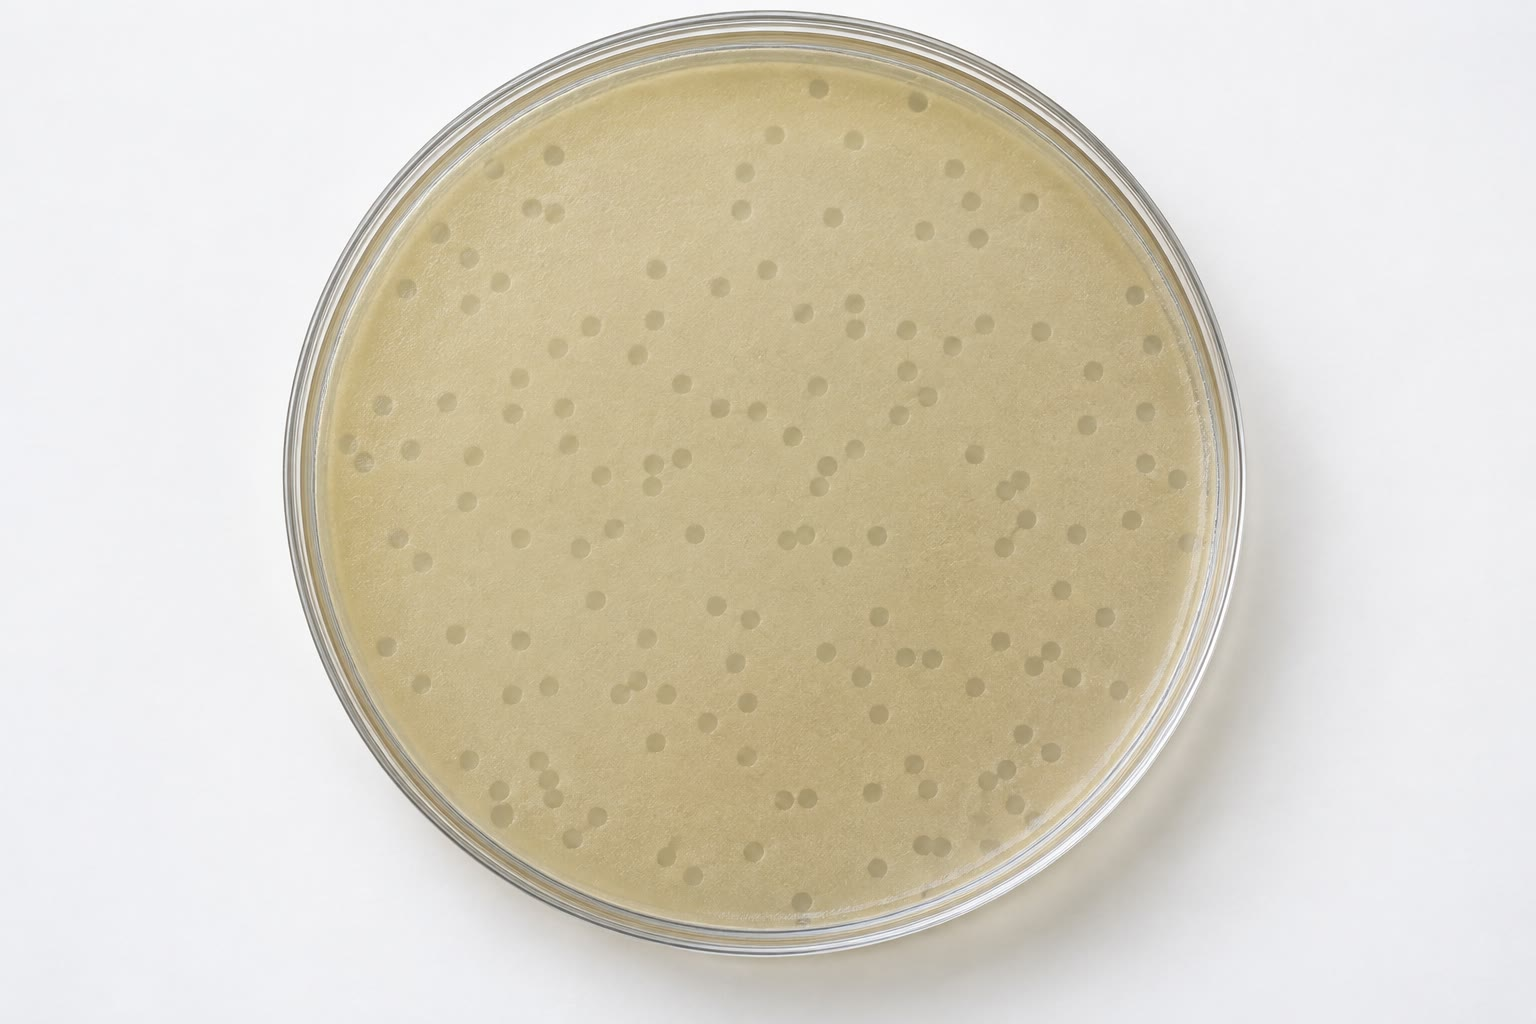
\includegraphics[width=0.46\linewidth]{images/book5/ai/b5-13-plaque-assay.jpg}\hspace{0.04\linewidth}
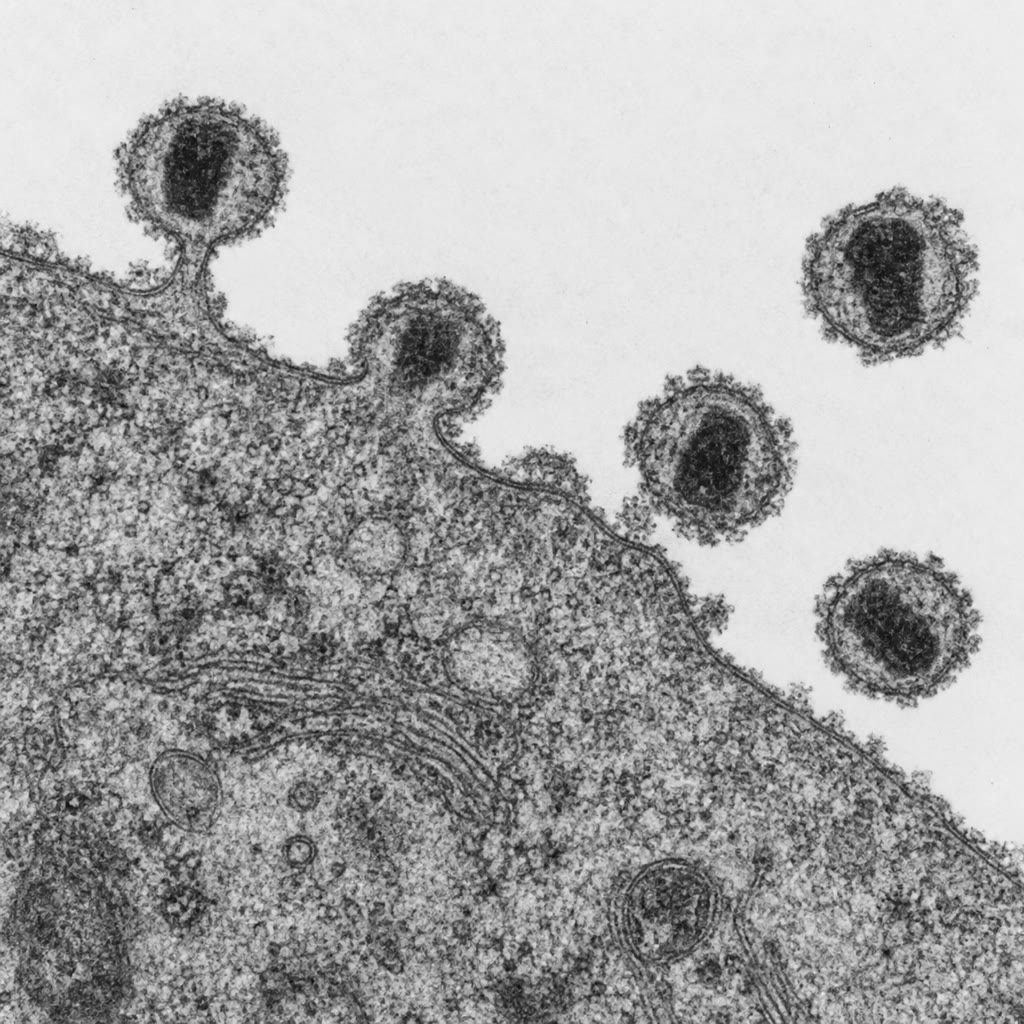
\includegraphics[width=0.36\linewidth]{images/book5/ai/b5-13-hiv-budding.jpg}

{\small 左：细菌菌苔中的噬斑，每个噬斑是一片透明区域，其中
一种噬菌体的子代已裂解了其周围的细胞。右：HIV
颗粒从 T~淋巴细胞出芽，其\omterm{def:b3:virology:virus}{包膜}取自
细胞膜。}
\end{omfigure}

\begin{theorem}[宿主内的感染动力学]\label{thm:b3:virology:dynamics}
\index{基本再生数!宿主内}\index{病毒载量}\index{病毒动力学}
设 $T$ 为易感靶细胞的密度，$I$ 为
被感染细胞的密度，$V$ 为游离\omterm{def:b3:virology:virus}{病毒粒子}的密度。\omterm{def:b3:virology:virus}{病毒粒子}以速率 $\beta TV$ 感染靶细胞，
被感染细胞以速率 $p$ 各自产生\omterm{def:b3:virology:virus}{病毒粒子}，并以速率
$\delta$ 死亡，游离\omterm{def:b3:virology:virus}{病毒粒子}以速率 $c$ 被清除：
\[
\frac{\mathrm{d}I}{\mathrm{d}t} = \beta TV - \delta I, \qquad
\frac{\mathrm{d}V}{\mathrm{d}t} = pI - cV .
\]
$T$ 保持恒定时，若\emph{基本
再生数} $R_{0} = \beta Tp/(c\delta)$ 大于 $1$，则感染增长；
稳态时 $V^{*} = p I^{*}/c$，产生与清除相平衡。
若药物在 $t = 0$ 时阻断一切新感染（$\beta \to 0$），则
\omterm{def:b3:virology:virus}{病毒粒子}起初以清除速率 $c$ 衰减，随后，
游离\omterm{def:b3:virology:virus}{病毒}降至剩余被感染细胞所维持的水平后，
则以这些细胞的死亡速率 $\delta$ 衰减：
\[
V(t) \approx V_{0}\,\frac{c\,e^{-\delta t} - \delta\,e^{-ct}}{c - \delta}
\;\longrightarrow\; V_{0}\,\frac{c}{c-\delta}\,e^{-\delta t}
\quad (t \gg 1/c).
\]
治疗后\omterm{thm:b3:virology:dynamics}{病毒载量}的两段斜率分别测得 $c$ 和
$\delta$，由 $pI^{*} = cV^{*}$ 可得治疗前\omterm{def:b3:virology:virus}{病毒粒子}的
每日产生量。
\end{theorem}
\begin{proof}
被感染细胞平均存活 $1/\delta$，平均产生 $p/\delta$
个\omterm{def:b3:virology:virus}{病毒粒子}；每个\omterm{def:b3:virology:virus}{病毒粒子}存活 $1/c$，并在其间感染 $\beta T/c$
个细胞，两者之积即一个被感染细胞所衍生的
被感染细胞数，即 $R_{0}$。稳态时 $\mathrm{d}V/\mathrm{d}t = 0$
可得 $V^{*} = pI^{*}/c$。治疗后 $\mathrm{d}I/\mathrm{d}t =
-\delta I$，故 $I = I_{0}e^{-\delta t}$，且 $\mathrm{d}V/\mathrm{d}t =
pI_{0}e^{-\delta t} - cV$ 为线性方程，其解满足
$V(0) = V_{0} = pI_{0}/c$ 的解即为所给表达式（检验：当 $t = 0$ 时，其值等于
$V_{0}$，且逐项满足方程）。当 $t
\gg 1/c$ 时，$e^{-ct}$ 项已消失，$V$ 随被感染细胞以斜率 $-\delta$ 变化；
当 $t \ll 1/\delta$ 且 $c \gg \delta$ 时，早期
斜率为 $-c$。
\end{proof}

\begin{example}[方程前后的 HIV]\label{ex:b3:virology:hiv}
直到 1995 年，HIV 感染的临床潜伏期——\omterm{thm:b3:virology:dynamics}{病毒载量}
稳定在每毫升 $10^{4}$--$10^{6}$ 拷贝，T~细胞缓慢减少——
被视为静止\omterm{def:b3:virology:virus}{病毒}。何大一、佩雷尔森及其同事
给患者服用\omterm{def:b3:virology:drugs}{蛋白酶抑制剂}，并将\omterm{thm:b3:virology:dynamics}{病毒载量}的下降
用该定理拟合：快速阶段给出 $c \approx \qty{3}{d^{-1}}$
（\omterm{def:b3:virology:virus}{病毒粒子}半衰期约六小时），慢速阶段给出 $\delta \approx
\qty{0.5}{d^{-1}}$（受感染细胞寿命约一天半）。
稳定的\omterm{thm:b3:virology:dynamics}{病毒载量}为每毫升 $10^{5}$，存在于 \qty{15}{L} 体液中，
以速率 $c$ 被清除，因此需每天产生约 $10^{10}$
个\omterm{def:b3:virology:virus}{病毒粒子}，日复一日持续数年：“潜伏”期是一种
感染与死亡激烈进行的稳态，T~细胞库
每日被补充，直至衰竭。下一节的突变计算
随即可得，并由此解释单药失效而
三药不然的原因。
\end{example}

\begin{omfigure}
\begin{tikzpicture}
\begin{axis}[
  width=0.7\linewidth, height=5.8cm,
  axis x line=bottom, axis y line=left,
  xmin=0, xmax=14, ymin=10, ymax=2e5, ymode=log,
  xlabel={开始治疗后的天数}, ylabel={每毫升病毒粒子数},
  xlabel style={font=\small, at={(axis description cs:0.5,-0.12)}, anchor=north}, ylabel style={font=\small},
  tick label style={font=\small}, xtick={0,2,4,6,8,10,12,14},
  clip=false,
]
\addplot[very thick, omDef, domain=0:14, samples=100] {1e5*(3*exp(-0.5*x) - 0.5*exp(-3*x))/2.5};
\addplot[dashed, omThm, domain=0:1.6, samples=2] {1e5*exp(-3*x)};
\addplot[dashed, omMeth!70!black, domain=1.5:14, samples=2] {1e5*1.2*exp(-0.5*x)};
\node[font=\scriptsize, omThm, anchor=west] at (axis cs:1.8,600) {游离病毒粒子被清除：斜率 $-c$，半衰期 \qty{6}{h}};
\node[font=\scriptsize, omMeth!70!black, anchor=south west] at (axis cs:5.5,1.5e4) {受感染细胞死亡：斜率 $-\delta$，半衰期 \qty{1.4}{d}};
\end{axis}
\end{tikzpicture}

{\small 药物阻止新感染后的\omterm{thm:b3:virology:dynamics}{病毒载量}，由定理给出，
取 $c = \qty{3}{d^{-1}}$，$\delta = \qty{0.5}{d^{-1}}$：游离\omterm{def:b3:virology:virus}{病毒粒子}被清除时
快速下降，随后是由原已感染细胞死亡
所控制的较慢下降。}
\end{omfigure}

\section{病毒如何演化}

\begin{definition}[突变、准种、漂移与转换]\label{def:b3:virology:evolution}
\index{准种}\index{抗原漂移}\index{抗原转换}\index{重配}
依赖 RNA 的聚合酶与逆转录酶不具备
\omterm{prop:b3:dna-repair:fidelity}{校对}功能，RNA \omterm{def:b3:virology:virus}{病毒}每个核苷酸每次复制的突变率为 $10^{-4}$ 至 $10^{-6}$——
比其宿主高出一千至一百万倍——
因此 RNA \omterm{def:b3:virology:virus}{病毒}种群是由一团
相关基因组构成的云团，即\emph{准种}；种群足够大时，其中每个单点
突变体始终存在。选择
由抗体施加，推动\emph{抗原漂移}：流感\omterm{def:b3:virology:virus}{病毒}的表面蛋白
逐年积累替换，去年获得的
免疫力每季保护作用都在减弱。\emph{抗原转换}是一次跳跃：一个
分节的基因组（流感\omterm{def:b3:virology:virus}{病毒}有八个 RNA 片段）可发生
\emph{重配}，若一个
片段编码来自禽类或猪\omterm{def:b3:virology:virus}{病毒}的血凝素，人类对其毫无免疫力，
便会引发大流行——1918、1957、1968、2009。
基因组内的重组对不分节的\omterm{def:b3:virology:virus}{病毒}也有同样作用，
而冠状\omterm{def:b3:virology:virus}{病毒}可自由重组。大多数新出现的人类\omterm{def:b3:virology:virus}{病毒}是
\emph{人兽共患病}，即从动物储库跨入人类——冠状\omterm{def:b3:virology:virus}{病毒}、埃博拉\omterm{def:b3:virology:virus}{病毒}和狂犬\omterm{def:b3:virology:virus}{病毒}的储库是蝙蝠；
流感来自禽类和猪；HIV 来自灵长类——
而跨越通常只需受体结合
蛋白上的几个突变。
\end{definition}

\begin{proposition}[错误阈值]\label{prop:b3:virology:error-threshold}
\index{错误阈值}\index{校对!病毒的}
长为 $L$ 个核苷酸、每个核苷酸复制错误率为 $u$ 的基因组，
无误复制的概率为 $(1-u)^{L} \approx e^{-uL}$。
若最适序列要在种群中抵御
其突变体的大量涌入而存续，则无误复制的比例必须超过
约为其选择优势 $\sigma$ 的倒数：$e^{-uL} \gtrsim
1/\sigma$，即 $uL \lesssim \ln\sigma$，数量级为 1。
故突变率与基因组长度的乘积有上界：一个
RNA \omterm{def:b3:virology:virus}{病毒}若 $u = 10^{-4}$，其基因组不可能远长于
$10^{4}$ 个核苷酸，这大致与 RNA \omterm{def:b3:virology:virus}{病毒}的实际相符；而
冠状\omterm{def:b3:virology:virus}{病毒}的基因组长达 \qty{30}{kb}，是已知最长的 RNA 基因组，
它们只能通过编码一种\omterm{prop:b3:dna-repair:fidelity}{校对}外切核酸酶、使 $u$ 降低十倍，才能达到这一长度。
阈值也可作为一种武器：提高聚合酶错误率的药物
（利巴韦林、莫努匹韦）可使\omterm{def:b3:virology:virus}{病毒}越过阈值，进入\emph{错误
\omterm{def:b3:cytoskeleton-motility:instability}{灾变}}，\omterm{def:b3:virology:evolution}{准种}随之崩溃。
\end{proposition}
\begin{proof}
各 $L$ 个位点的错误相互独立，故无误概率为
$(1-u)^{L}$，且 $\ln(1-u) \approx -u$ 在 $u$ 较小时成立。种群
平衡由标准的\omterm{def:b3:virology:evolution}{准种}论证给出（艾根，1971）：主序列
以速率 $\sigma e^{-uL}$ 相对于平均突变体得到补充，
否则因突变而损失；只有当前者
超过 $1$ 时才能维持，由此得到上界。
\end{proof}

\begin{omfigure}
\begin{tikzpicture}[every node/.style={font=\scriptsize}, >=stealth]
  % drift
  \begin{scope}
    \foreach \i in {0,1,2,3} { \draw[thick, omProp, fill=omProp!30] (\i*1.3,0) circle (0.35); \foreach \a in {0,60,...,300} \draw[omProp, thick] (\i*1.3,0) ++(\a:0.35) -- ++(\a:0.14); }
    \foreach \i/\n in {1/1,2/2,3/3} { \foreach \k in {1,...,\n} \fill[omThm] (\i*1.3,0) ++({60*\k+20}:0.5) circle (0.06); }
    \foreach \i in {0,1,2} \draw[->, thick] (\i*1.3+0.5,0) -- (\i*1.3+0.8,0);
    \node[below, align=center] at (1.95,-0.6) {抗原漂移：点突变在 \\表面蛋白中逐季积累};
  \end{scope}
  % shift
  \begin{scope}[xshift=7.0cm]
    \draw[thick, omProp, fill=omProp!30] (0,0.5) circle (0.4); \foreach \y in {-0.2,-0.1,0,0.1,0.2} \draw[omProp!80!black] (-0.25,0.5+\y) -- (0.25,0.5+\y);
    \draw[thick, omMeth!70!black, fill=omMeth!30] (0,-0.7) circle (0.4); \foreach \y in {-0.2,-0.1,0,0.1,0.2} \draw[omMeth!70!black] (-0.25,-0.7+\y) -- (0.25,-0.7+\y);
    \node[left, align=right] at (-0.5,0.5) {人类毒株，\\8 个片段}; \node[left, align=right] at (-0.5,-0.7) {禽类毒株，\\8 个片段};
    \draw[->, thick] (0.5,0.4) -- (1.5,0.0); \draw[->, thick] (0.5,-0.6) -- (1.5,-0.2);
    \draw[thick, omDef, fill=omDef!10] (2.4,-0.1) ellipse (0.9 and 0.7); \node[below] at (2.4,-0.85) {一头猪的一个细胞};
    \draw[->, thick] (3.4,-0.1) -- (4.3,-0.1);
    \draw[thick, omProp, fill=omProp!30] (4.9,-0.1) circle (0.4); \foreach \y in {-0.2,-0.1,0.1,0.2} \draw[omProp!80!black] (4.65,-0.1+\y) -- (5.15,-0.1+\y); \draw[omMeth!70!black, very thick] (4.65,-0.1) -- (5.15,-0.1);
    \node[right, align=left] at (5.4,-0.1) {重配病毒：禽类 \\血凝素存于 \\人类病毒中};
    \node[below, align=center] at (2.4,-1.5) {抗原转换：整个片段被交换；\\无人免疫——即大流行};
  \end{scope}
\end{tikzpicture}

{\small 流感\omterm{def:b3:virology:virus}{病毒}逃避免疫有两种方式。\omterm{def:b3:virology:evolution}{抗原漂移}：
刺突蛋白中的突变逐渐积累。\omterm{def:b3:virology:evolution}{抗原转换}：同一细胞中的两个毒株
交换整套基因组片段，一种人类此前未见的刺突蛋白
随即一次性出现。}
\end{omfigure}

\begin{example}[为何 HIV 需要三种药物]\label{ex:b3:virology:three-drugs}
HIV 的逆转录酶约每 $10^{5}$ 个核苷酸出错一次，因此
每次复制的 \qty{9700}{nt} 基因组平均携带约 $0.1$ 个突变，而
每天新产生的 $10^{10}$ 个基因组共携带 $10^{9}$ 个突变：
$3\times 9700 \approx \num{30000}$ 种可能的单点
突变中，每一种在给药前每天都会出现多次。一种药物若能被单个
突变即可击败——正如单个突变能击败多数逆转录酶和
\omterm{def:b3:virology:drugs}{蛋白酶抑制剂}——因此会在数周内被击败，
1987 年的 AZT 正是如此。两个独立突变
同时出现的频率为每个基因组 $10^{-10}$，约每天一次；
三个突变则为 $10^{-15}$，千天一次——而一名服用三种
药物且\omterm{thm:b3:virology:dynamics}{病毒载量}已下降千倍的患者，每天仅产生 $10^{7}$ 个基因组，
因此三重突变体从不出现。这一点，加上该定理所证明的
\omterm{def:b3:virology:virus}{病毒}正以最快速度复制，使自 1996 年起的\omterm{thm:b3:cancer-biology:goldie-coldman}{联合疗法}
成为将艾滋病转为
慢性病的治疗手段。
\end{example}

\section{宿主、防御与药物}

\begin{proposition}[致病机制与防御]\label{prop:b3:virology:pathogenesis}
\index{细胞病变效应}\index{干扰素}\index{限制!噬菌体}
\omterm{def:b3:virology:virus}{病毒}通过裂解细胞致病（脊髓灰质炎破坏运动神经元，HIV 杀死
T~细胞），通过使细胞产生有毒产物致病，通过使细胞转化
（见\cref{ch:b3:cancer-biology}），并且往往主要通过宿主自身的
反应致病：发热、组织\omterm{def:b3:dna-repair:lesions}{损伤}，以及最严重时
由流感或 SARS 冠状\omterm{def:b3:virology:virus}{病毒}引发的免疫反应，即细胞因子风暴。宿主
以先天防御识别\omterm{def:b3:virology:virus}{病毒}复制的
特征——双链 RNA、无帽 RNA、
胞质中的 DNA——并以\emph{\omterm{prop:b3:virology:pathogenesis}{干扰素}}作出反应，使每个
邻近细胞进入抗\omterm{def:b3:virology:virus}{病毒}状态（见\cref{ch:b3:innate-immunity}）；
自然杀伤细胞可摧毁已隐藏 MHC 的细胞；
以抗体中和\omterm{def:b3:virology:virus}{病毒粒子}，以细胞毒性 T~细胞杀死感染细胞
使其在释放子代之前被清除（见\cref{ch:b3:adaptive-immunity}）；
在细菌中，以\omterm{def:b3:genetic-engineering:tools}{限制酶}切割外源 DNA，并以
\cref{ch:b3:genetic-engineering}中的 \omterm{def:b3:genetic-engineering:crispr}{CRISPR} 记忆来防御。\omterm{def:b3:virology:virus}{病毒}也会反击：
几乎所有大型\omterm{def:b3:virology:virus}{病毒}都编码能阻断\omterm{prop:b3:virology:pathogenesis}{干扰素}、隐藏
MHC、模拟细胞因子或抑制\omterm{def:b3:cell-cycle-apoptosis:apoptosis}{细胞凋亡}的蛋白质，这场军备竞赛
被同时写入双方的基因组之中。
\end{proposition}

\begin{definition}[抗病毒药物与疫苗]\label{def:b3:virology:drugs}
\index{抗病毒药物}\index{核苷类似物}\index{蛋白酶抑制剂}\index{疫苗}\index{mRNA 疫苗}
抗\omterm{def:b3:virology:virus}{病毒}药物攻击\omterm{def:b3:virology:virus}{病毒}的酶，或攻击宿主细胞
自身不进行的步骤。\emph{核苷类似物}是\omterm{def:b3:genomics:sanger}{链终止}剂：阿昔洛韦
仅被疱疹\omterm{def:b3:virology:virus}{病毒}胸苷激酶磷酸化，随后
阻断\omterm{def:b3:virology:virus}{病毒} DNA 聚合酶，因此只在感染细胞中起作用；
AZT、替诺福韦和拉米夫定阻止逆转录酶；瑞德西韦和
莫努匹拉韦作用于冠状\omterm{def:b3:virology:virus}{病毒}聚合酶，后者通过
诱变起作用。\emph{蛋白酶抑制剂}阻断\omterm{def:b3:virology:virus}{病毒}多聚蛋白的切割
（HIV、丙型肝炎\omterm{def:b3:virology:virus}{病毒}、SARS-CoV-2 的奈玛特韦）。整合酶
抑制剂阻止 HIV 前\omterm{def:b3:virology:virus}{病毒}的形成；神经氨酸酶抑制剂阻止
流感\omterm{def:b3:virology:virus}{病毒粒子}从其出芽的细胞上脱离；进入抑制剂
阻断受体。丙型肝炎\omterm{def:b3:virology:virus}{病毒}现在十二周即可被治愈，
方法是联合使用直接作用药物，这是首例被化学疗法治愈的
慢性\omterm{def:b3:virology:virus}{病毒}感染。\emph{疫苗}提供
\omterm{def:b3:virology:virus}{病毒}抗原，而不引起其疾病：减毒活\omterm{def:b3:virology:virus}{病毒}（麻疹、
口服脊髓灰质炎疫苗、黄热病），灭活\omterm{def:b3:virology:virus}{病毒}（注射用脊髓灰质炎疫苗、
流感），亚单位（在酵母中制备的乙型肝炎表面抗原、
乳头瘤\omterm{def:b3:virology:virus}{病毒}\omterm{def:b3:virology:virus}{衣壳}蛋白），以及一种无害的\omterm{def:b3:virology:virus}{病毒}载体，携带
目标的基因，或自 2020 年起的\emph{信使 RNA}，其编码
抗原，经脂质纳米颗粒递送，由接种者自身的细胞
翻译。它们为何有效，以及需要接种多少人才能保护
其余人群，其免疫学原理
在\cref{ch:b3:adaptive-immunity}中讨论。
\end{definition}

\begin{remark}[生命经济中的病毒]\label{rem:b3:virology:economy}
危害人类的\omterm{def:b3:virology:virus}{病毒}在世界\omterm{def:b3:virology:virus}{病毒}种群中
微不足道，其中大多数感染细菌和古菌。噬菌体每天杀死
海洋中五分之一至三分之一的细菌，并将其内容物
释放回溶解态储库——即\emph{\omterm{def:b3:virology:virus}{病毒}分流}，属于
本科二年级分册中的碳循环。它们在细菌之间\omterm{def:b3:cancer-biology:hallmarks}{转移}基因
（见\cref{ch:b3:bacteriology}），其毒素与白喉、霍乱
和最恶劣的\emph{E.~coli}的毒素相同。人类基因组的 8\%
是古老逆转录\omterm{def:b3:virology:virus}{病毒}的遗存，
（见\cref{ch:b3:genomics}），其中一个\omterm{def:b3:virology:virus}{包膜}基因现在使
胎盘细胞融合。\omterm{def:b3:virology:virus}{病毒}是地球上遗传新颖性的最大储库，
而何为活的界限
正穿过\omterm{def:b3:virology:virus}{病毒}。
\end{remark}

\section{练习}

\begin{exercise}[$\star$]\label{exo:b3:virology:1}
将脊髓灰质炎\omterm{def:b3:virology:virus}{病毒}、流感\omterm{def:b3:virology:virus}{病毒}、HIV、单纯疱疹\omterm{def:b3:virology:virus}{病毒}、乙型肝炎\omterm{def:b3:virology:virus}{病毒}与轮状\omterm{def:b3:virology:virus}{病毒}
归入其\omterm{def:b3:virology:virus}{巴尔的摩分类}，并说明每种\omterm{def:b3:virology:virus}{病毒}必须携带或产生、而细胞所缺乏的
是哪一种酶。
\end{exercise}

\begin{exercise}[$\star$]\label{exo:b3:virology:2}
赫尔希–蔡斯实验说明了什么？若蛋白质携带遗传指令，
又会得到什么结果？
\end{exercise}

\begin{exercise}[$\star$]\label{exo:b3:virology:3}
噬菌体原液稀释 $10^{-7}$ 后，取 \qty{0.1}{mL} 得到 $84$ 个噬斑。
该噬菌体的效价是多少？为何电子显微镜
计得的颗粒数可能多出十倍？
\end{exercise}

\begin{exercise}[$\star$]\label{exo:b3:virology:4}
列出复制周期的六个阶段，并针对每个阶段
指出一种作用于它的\omterm{def:b3:virology:drugs}{抗病毒药物}或宿主防御。
\end{exercise}

\begin{exercise}[$\star\star$]\label{exo:b3:virology:5}
利用 \cref{prop:b3:virology:economy}，计算
编码由 $180$ 个拷贝的
\qty{30}{kDa} 蛋白组成的\omterm{def:b3:virology:virus}{病毒}\omterm{def:b3:virology:virus}{衣壳}所需的核酸量，并与此类\omterm{def:b3:virology:virus}{病毒}可能拥有的
\qty{4.5}{kb} 基因组进行比较。\omterm{def:b3:virology:virus}{衣壳}基因占基因组的比例是多少？
\end{exercise}

\begin{exercise}[$\star\star$]\label{exo:b3:virology:6}
设 $c = \qty{3}{d^{-1}}$，$\delta = \qty{0.5}{d^{-1}}$，$V_{0} =
10^{5}$ 每毫升，由定理计算 $V$ 在 $t = 0.5$、$2$ 和
$10$ 天时的值。\omterm{thm:b3:virology:dynamics}{病毒载量}需多久才降至
$50$ 每毫升（检出限）以下？
\end{exercise}

\begin{exercise}[$\star\star$]\label{exo:b3:virology:7}
某 RNA \omterm{def:b3:virology:virus}{病毒}的 $u = 3\times 10^{-5}$，$L = \qty{12}{kb}$。
其子代基因组中不携带突变的比例是多少？若某诱变药物使 $u$
增至三倍，该比例将如何变化？试说明冠状\omterm{def:b3:virology:virus}{病毒}为何需要
一种\omterm{prop:b3:dna-repair:fidelity}{校对}酶。
\end{exercise}

\begin{exercise}[$\star\star$]\label{exo:b3:virology:8}
试说明流感中的\omterm{def:b3:virology:evolution}{抗原漂移}与\omterm{def:b3:virology:evolution}{抗原转换}，以及为何迄今为止
每一株大流行毒株都携带一种新的血凝素。
\end{exercise}

\begin{exercise}[$\star\star$]\label{exo:b3:virology:9}
阿昔洛韦是一种鸟苷类似物，须先经磷酸化才能发挥作用。
试说明它为何只\omterm{def:b3:dna-repair:lesions}{损伤}疱疹\omterm{def:b3:virology:virus}{病毒}感染的细胞而不\omterm{def:b3:dna-repair:lesions}{损伤}其他细胞，并预测
耐药突变。
\end{exercise}

\begin{exercise}[$\star\star\star$]\label{exo:b3:virology:10}
由定理中的两个方程推导 $R_{0} = \beta Tp/(c\delta)$，
即求小规模感染（$I$、$V$ 接近零，$T$ 恒定）增长的条件，
并解释每个因子的含义。
\end{exercise}

\begin{exercise}[$\star\star\star$]\label{exo:b3:virology:11}
一名接受有效治疗的患者体内仍有 $10^{6}$ 个
前\omterm{def:b3:virology:virus}{病毒}沉默的潜伏感染静息 T~细胞，半衰期为
$44$ 个月。要使储库降至一个细胞以下，治疗需持续多久？
为何这使得 HIV 无法被仅阻断复制的药物治愈，
治愈需要满足什么条件？
\end{exercise}

\begin{exercise}[$\star\star\star$]\label{exo:b3:virology:12}
解释\cref{ex:b3:virology:three-drugs}的论证，
并用你自己的数字，针对一种基因组为 \qty{30}{kb}、$u = 10^{-6}$ 的\omterm{def:b3:virology:virus}{病毒}，
每天产生 $10^{9}$ 个基因组。你会联合几种药物？为何作用于同一种酶
两个位点的药物不能算作两种？
\end{exercise}

\section{问题：患者体内的病毒}

\begin{problem}[{周末问题——逐个病毒粒子计数的 HIV 感染，
其动力学拟合治疗曲线，突变按药物统计，
其储库的衰减时间经测定，
最后归结为每日产生的病毒粒子数、病毒载量变为不可检出的那一天，
以及三重突变体存在的概率}]
\label{pb:b3:virology:1}
数据：患者体内\omterm{thm:b3:virology:dynamics}{病毒载量} $V^{*} = 2\times 10^{5}$ 每毫升，
体液共 \qty{15}{L}；$c = \qty{3}{d^{-1}}$，$\delta = \qty{0.5}{d^{-1}}$；每个感染细胞每天产生
$p = 500$ 个\omterm{def:b3:virology:virus}{病毒粒子}；基因组 \qty{9700}{nt}，$u = 10^{-5}$
每个核苷酸每次复制；单个突变即可使\omterm{def:b3:virology:virus}{病毒}对
三种药物中的每一种产生耐药性；三联治疗时产量降至
$10^{7}$ 个基因组每天；潜伏储库 $10^{6}$ 个细胞，半衰期 $44$ 个月；
一个\omterm{def:b3:virology:virus}{病毒粒子}为直径 \qty{120}{nm} 的球体，内含两条 \qty{9700}{nt} 的 RNA
链及约 \num{2000} 个 \qty{25}{kDa} 的蛋白质分子。

\medskip
\noindent\textbf{第一部分——计数。}
\begin{enumerate}
  \item 处于稳态时，体内有多少个\omterm{def:b3:virology:virus}{病毒粒子}？
  \item 每天清除多少个，由此每天产生多少个？
  \item 多少个感染细胞产生这些\omterm{def:b3:virology:virus}{病毒粒子}，
        每天有多少个细胞死亡？
  \item 一个\omterm{def:b3:virology:virus}{病毒粒子}的质量为多少（RNA 按每个核苷酸 \qty{330}{Da} 计，
        加上蛋白质），体内\omterm{def:b3:virology:virus}{病毒粒子}的总质量是多少？
        并与一粒沙子（\qty{1}{mg}）作比较。
  \item 人体有 $10^{12}$ 个 CD4 T~细胞，并替换其中
        被感染的细胞。任一时刻感染细胞占细胞库的比例是多少，
        这一微小比例如何能在十年内杀死整个细胞库？
  \item 若每个感染细胞通过\omterm{def:b3:cell-cycle-apoptosis:apoptosis}{细胞凋亡}死亡，并在
        一小时内被吞噬（见\cref{ch:b3:cell-cycle-apoptosis}），
        任一时刻有多少个正在被清除？
\end{enumerate}

\medskip
\noindent\textbf{第二部分——治疗。}
\begin{enumerate}[resume]
  \item 治疗于 $t = 0$ 时阻止新感染。由定理计算 $V$ 在 $t =
        1$、$3$、$7$ 和 $14$ 天时的值。
  \item \omterm{thm:b3:virology:dynamics}{病毒载量}在哪一天降至
        检出限 $50$ 每毫升以下？
  \item 由两段斜率，临床医生如何估计 $c$ 与
        $\delta$，需根据第 $0$--$1$ 天和第 $3$--$10$ 天的测量数据？
  \item 两个阶段之后，\omterm{thm:b3:virology:dynamics}{病毒载量}趋于平稳，每毫升仅数个拷贝，
        并在此水平维持数年。模型中缺失的是哪一个房室，
        其衰减速率是多少？
  \item 计算游离\omterm{def:b3:virology:virus}{病毒粒子}和感染细胞的半衰期。
  \item 试说明治疗前的平台期为何被误读为潜伏，
        而方程实际揭示了什么？
\end{enumerate}

\medskip
\noindent\textbf{第三部分——突变。}
\begin{enumerate}[resume]
  \item 每次复制每个基因组的突变数，以及未治疗患者
        每天产生的突变数。
  \item 基因组中可能存在多少种不同的单点突变？
        每种突变每天出现多少次？
  \item 某一特定双突变体和某一特定三突变体的每基因组发生率，
        未治疗时每天各产生多少个？
  \item 三联治疗、每天 $10^{7}$ 个基因组的情况下，
        每年预期产生多少个三突变体？
  \item 患者漏服药物，使其中一种药物浓度降至零达一周，
        另外两种药物仍有效。哪些突变体现在可以被选择，
        以及这一周内相关双突变体的期望
        产生数（每天 $10^{7}$ 个基因组）
        是多少？
  \item 为何对一种\omterm{def:b3:virology:drugs}{核苷类似物}的耐药性往往也赋予
        对另一种的耐药性，这又如何改变
        “独立”药物的数目？
\end{enumerate}

\medskip
\noindent\textbf{第四部分——储库与治愈。}
\begin{enumerate}[resume]
  \item 半衰期为 $44$ 个月，$10^{6}$ 个潜伏细胞
        降至一个需多久？降至 $10^{4}$ 个呢？
  \item 若停止治疗，一个潜伏细胞重新激活即足以
        重新引发感染。停药后，\omterm{thm:b3:virology:dynamics}{病毒载量}需多久
        才回升至每毫升 $10^{5}$（若\omterm{def:b3:virology:virus}{病毒}以每代 $R_{0} = 8$、
        每代历时 $2$ 天、从一个\omterm{def:b3:virology:virus}{病毒粒子}起增长）？
  \item 基于该模型提出两种治愈策略，
        并指出各自的障碍。
  \item 定理中的 $R_{0}$ 仅针对宿主体内。HIV 在人与人之间的
        人群 $R_{0}$ 约为 $3$--$5$。须阻止多大比例的
        传播，才能终结疫情
        （$1 - 1/R_{0}$）？
  \item 治疗几乎将患者的传播性降至零。试说明
        “治疗即预防”如何由
        体内定理推出。
  \item 效力为 $E$（即接种者中受保护的比例）的\omterm{def:b3:virology:drugs}{疫苗}，
        若接种于人群中 $f$ 的比例，则可保护人群中
        $Ef$ 的比例。要达到上一问的阈值，需要多大的接种覆盖率 $f$？
        在 $E = 0.7$ 与 $E = 0.9$ 时各需多大？第一个答案
        意味着什么？
  \item 汇总：每天产生的\omterm{def:b3:virology:virus}{病毒粒子}数（第~2~问），\omterm{thm:b3:virology:dynamics}{病毒载量}
        变为不可检出的那一天（第~8~问），以及治疗期间
        每年三突变体的期望数（第~16~问）。
\end{enumerate}
\end{problem}
